\section[Fault Tolerance]{Theme 1: Fault Tolerance}

\begin{frame}
  \frametitle{Research Topic 1: Fault Tolerance}

  Two complementary approaches to \textcolor{blue}{Fault Tolerance}

  \bigskip

  \begin{tabular}{p{.45\linewidth}|p{.45\linewidth}}
    General Purpose Fault Tolerance     & Application-Specific Fault Tolerance \\
    &\\\hline
    &\\
    \begin{minipage}{\linewidth}
      \begin{itemize}
      \item Checkpointing and rollback-recovery
      \item How to checkpoint (protocols)
      \item When to checkpoint
      \end{itemize}
    \end{minipage} & \begin{minipage}{\linewidth}
      \begin{itemize}
      \item Middleware to enable writing FT applications
      \item Resilient algorithms
      \item How to build a resilient application
      \end{itemize}
    \end{minipage}
  \end{tabular}
\end{frame}


\begin{frame}
  \frametitle{Major Contribution 1: Enabling fault-tolerant MPI applications}

  \begin{columns}
    \begin{column}{.4\textwidth}
      \begin{minipage}{\linewidth}
        \begin{center}
          
\includegraphics[width=.9\linewidth]{MPIlogo.jpg}
          
          Message Passing Interface
        \end{center}
        \begin{itemize}
        \item De-facto standard of parallel programming in HPC
        \item $>99\%$ of HPC applications
        \item Available on all HPC systems
          \begin{itemize}
          \item vendor implementations based on either Open MPI or MPICH
          \end{itemize}
        \end{itemize}
      \end{minipage}
    \end{column}\begin{column}{.7\linewidth}
      Support for process failures in MPI:
      \begin{itemize}
      \item Until 2020 no support to tolerate failures\\
        Process crash $\Rightarrow$ communication failure \\
        communication failure $\Rightarrow$ MPI error \\
        MPI error $\Rightarrow$ interruption of the whole application / undefined behavior
      \item User-Level Failure Mitigation:\\
        \begin{itemize}
        \item A proposal to change the MPI standard to enable writing fault-tolerant applications
        \item An experimental implementation based on Open MPI
        \item Leading ideas:
          \begin{itemize}
          \item Minimal change of the MPI specification
          \item Addition of resilient features: failure detection, group membership, reliable broadcast, consensus
          \end{itemize}
        \end{itemize}
      \end{itemize}      
    \end{column}
  \end{columns}
  
\end{frame}

\begin{frame}
  \frametitle{My contributions related to ULFM}
  
  My major contributions related to ULFM:
  \begin{itemize}
  \item Co-designer of the ULFM specification \\
    $\Longrightarrow$\textcolor{red}{MPI Standard}
  \item Routines for the implementation of ULFM
    \begin{itemize}
    \item Failure Detector ($\Rightarrow$\textcolor{red}{best paper finalist SC'16})
    \item Consensus routine 
    \end{itemize}
  \item New application-specific fault-tolerant algorithms
    \begin{itemize}
    \item ABFT algorithms for matrix factorizations
    \item Managing process attrition in moldable applications
    \end{itemize}
  \item New composition technique of fault-tolerant approaches
  \end{itemize}

  ULFM software available by default on all HPC systems -- \textcolor{red}{integration in MPICH and Open MPI}
  
  Significant impact in the research community: $>10$ external projects depend on ULFM; highly cited research
\end{frame}

\section[Task-Based Runtime Systems]{Theme 2: Task-Based Runtime Systems}

\begin{frame}
  \frametitle{Research Topic 2: Task-Based Runtime Systems for HPC}

  \textcolor{brown}{Task Based Runtime Systems}
  \begin{itemize}
  \item Main question: how to reach performance portability in modern HPC architectures
    \begin{itemize}
    \item Networks with deep hierarchies / Manycore / NUMA / Accelerators
    \item Separation of concerns: going beyond MPI+X
    \item Management of asynchrony
    \item Overlap of computations and data movement
    \end{itemize}
  \item Related topics:
    \begin{itemize}
    \item Expression of parallelism / Programming Interfaces
    \item Out-of-(accelerator) core memory programming / Memory-Constrained algorithms
    \item Multiresolution computation with dynamic decision
    \item Sparse and computation-dependent task systems
    \end{itemize}
  \end{itemize}

\end{frame}


\begin{frame}
  \frametitle{Major Contribution 2: Task-Based Runtime Systems}

  \begin{columns}
    \begin{column}{.4\textwidth}
      \begin{minipage}{\linewidth}
        \begin{center}
          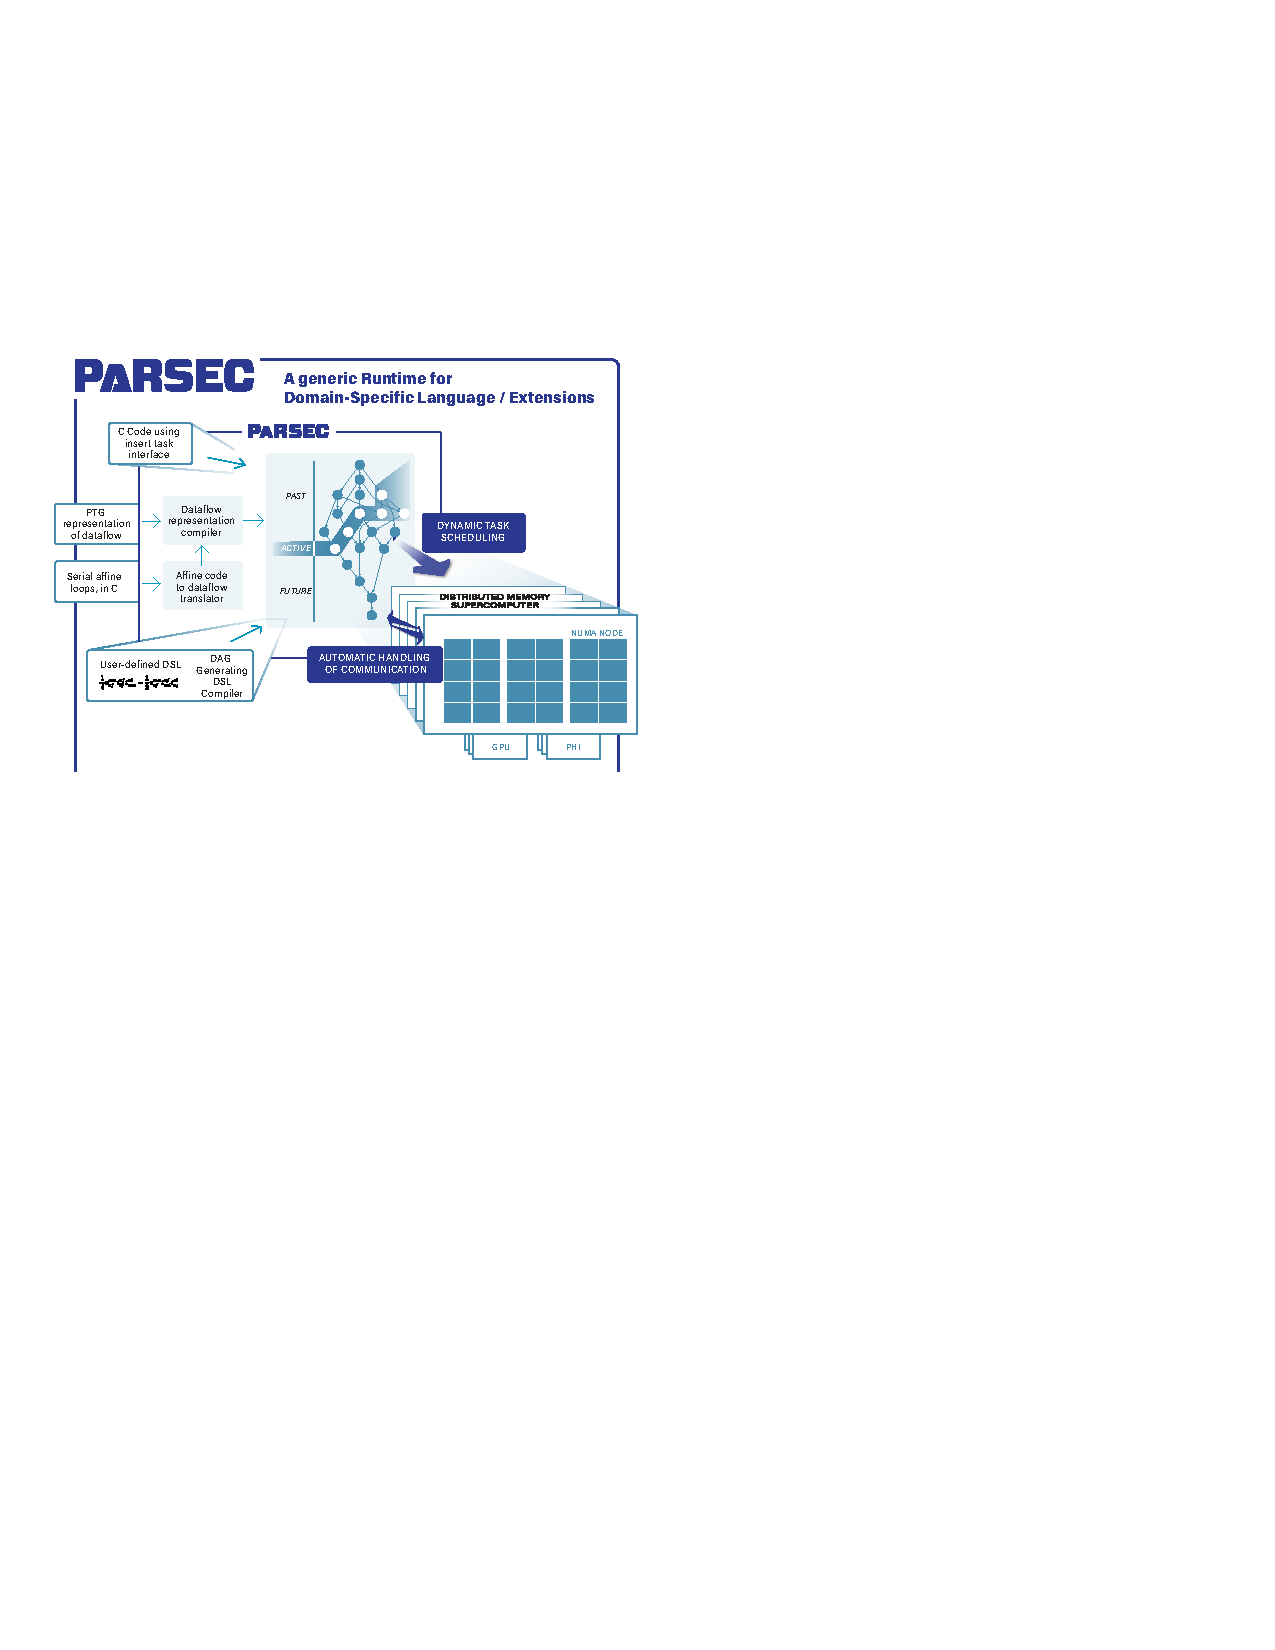
\includegraphics[width=.9\linewidth]{../parsec.pdf}
          
          \scriptsize PaRSEC: Parallel Runtime Scheduler and Execution Control
        \end{center}
        \begin{itemize}\scriptsize
        \item Task system for many micro tasks
        \item targets hybrid distributed large scale systems (e.g. Frontier)
        \item Available on all HPC systems via the Exascale Computing Project packages
        \end{itemize}
      \end{minipage}
    \end{column}\begin{column}{.7\linewidth}
      Support for task-based expression and execution in HPC
      \begin{itemize}
      \item How to manage asynchronous progress (of work, of communications)
      \item Promote separation of concerns: Algorithm expresses maximum parallelism, runtime maps to hardware
      \item Manage data hosting transparently (move data between nodes or devices in the background)
      \end{itemize}

      \bigskip

      \scriptsize PaRSEC software
      \begin{itemize}
      \item Provides various interfaces to program task systems (DSL, traditional 'insert-task' API, templated C++ interface for dynamic / computation-dependent DAGs)
      \item Comes with an ecosystem of tools (performance visualization, debugging)
      \end{itemize}
    \end{column}
  \end{columns}
  
\end{frame}

\begin{frame}
  \frametitle{My contributions related to PaRSEC}
  
  My major contributions related to \textcolor{brown}{PaRSEC}:
  \begin{itemize}
  \item Co-designer of the core engine
  \item Dynamic task schedulers, accelerator management
  \item Programming Interfaces 
    \begin{itemize}
    \item (Parameterized Task Graphs; Dynamic Task Discovery; Template Task Graphs)
    \end{itemize}
  \item Distributed Algorithms using or for PaRSEC
    \begin{itemize}
    \item Termination detection 
    \item Data redistribution
    \item Dense Linear Algebra
    \item Sparse Tensor Contraction -- \textcolor{red}{Application to Quantum Chemistry} 
    \end{itemize}
  \item Soft errors resilience in Task Systems
  \item Profiling and performance analysis ecosystem
  \end{itemize}
  
  PaRSEC software available by default on all HPC systems via the ECP packaging
  
  Significant impact on multiple communities (HiCMA -- \textcolor{red}{Gordon Bell finalist in 2022 with PaRSEC}; NWChemEX; MADNESS; MPQC; TiledArray; Chameleon; PASTiX)
    
\end{frame}
